\documentclass[hidelinks,12pt]{article}
\usepackage[left=0.25cm,top=1cm,right=0.25cm,bottom=1cm]{geometry}
%\usepackage[landscape]{geometry}
\textwidth = 20cm
\hoffset = -1cm
\usepackage[utf8]{inputenc}
\usepackage[spanish,es-tabla, es-lcroman]{babel}
\usepackage[autostyle,spanish=mexican]{csquotes}
\usepackage[tbtags]{amsmath}
\usepackage{nccmath}
\usepackage{amsthm}
\usepackage{amssymb}
\usepackage{mathrsfs}
\usepackage{graphicx}
\usepackage{subfig}
\usepackage{caption}
%\usepackage{subcaption}
\usepackage{standalone}
\usepackage[outdir=./Imagenes/]{epstopdf}
\usepackage{siunitx}
\usepackage{physics}
\usepackage{color}
\usepackage{float}
\usepackage{hyperref}
\usepackage{multicol}
\usepackage{multirow}
%\usepackage{milista}
\usepackage{anyfontsize}
\usepackage{anysize}
%\usepackage{enumerate}
\usepackage[shortlabels]{enumitem}
\usepackage{capt-of}
\usepackage{bm}
\usepackage{mdframed}
\usepackage{relsize}
\usepackage{placeins}
\usepackage{empheq}
\usepackage{cancel}
\usepackage{pdfpages}
\usepackage{wrapfig}
\usepackage[flushleft]{threeparttable}
\usepackage{makecell}
\usepackage{fancyhdr}
\usepackage{tikz}
\usepackage{bigints}
\usepackage{menukeys}
\usepackage{tcolorbox}
\tcbuselibrary{breakable}
\usepackage{scalerel}
\usepackage{pgfplots}
\usepackage{pdflscape}
\pgfplotsset{compat=1.16}
\spanishdecimal{.}
\renewcommand{\baselinestretch}{1.5} 
\renewcommand\labelenumii{\theenumi.{\arabic{enumii}})}

\newcommand{\python}{\texttt{python}}
\newcommand{\textoazul}[1]{\textcolor{blue}{#1}}
\newcommand{\azulfuerte}[1]{\textcolor{blue}{\textbf{#1}}}
\newcommand{\funcionazul}[1]{\textcolor{blue}{\textbf{\texttt{#1}}}}

\newcommand{\pderivada}[1]{\ensuremath{{#1}^{\prime}}}
\newcommand{\sderivada}[1]{\ensuremath{{#1}^{\prime \prime}}}
\newcommand{\tderivada}[1]{\ensuremath{{#1}^{\prime \prime \prime}}}
\newcommand{\nderivada}[2]{\ensuremath{{#1}^{(#2)}}}


\newtheorem{defi}{{\it Definición}}[section]
\newtheorem{teo}{{\it Teorema}}[section]
\newtheorem{ejemplo}{{\it Ejemplo}}[section]
\newtheorem{propiedad}{{\it Propiedad}}[section]
\newtheorem{lema}{{\it Lema}}[section]
\newtheorem{cor}{Corolario}
\newtheorem{ejer}{Ejercicio}[section]

\newlist{milista}{enumerate}{2}
\setlist[milista,1]{label=\arabic*)}
\setlist[milista,2]{label=\arabic{milistai}.\arabic*)}
\newlength{\depthofsumsign}
\setlength{\depthofsumsign}{\depthof{$\sum$}}
\newcommand{\nsum}[1][1.4]{% only for \displaystyle
    \mathop{%
        \raisebox
            {-#1\depthofsumsign+1\depthofsumsign}
            {\scalebox
                {#1}
                {$\displaystyle\sum$}%
            }
    }
}
\def\scaleint#1{\vcenter{\hbox{\scaleto[3ex]{\displaystyle\int}{#1}}}}
\def\scaleoint#1{\vcenter{\hbox{\scaleto[3ex]{\displaystyle\oint}{#1}}}}
\def\scaleiiint#1{\vcenter{\hbox{\scaleto[3ex]{\displaystyle\iiint}{#1}}}}
\def\bs{\mkern-12mu}

\newcommand{\Cancel}[2][black]{{\color{#1}\cancel{\color{black}#2}}}



\author{M. en C. Gustavo Contreras Mayén. \texttt{gux7avo@ciencias.unam.mx}}
\title{Evaluación del Examen Tema 5 - Métodos Monte Carlo \\ {\large Curso Física Computacional}}
\date{ }
\begin{document}

\maketitle
\fontsize{14}{14}\selectfont

\section{Problema 1.}
\begin{enumerate}
\item Propones un valor $b = 1000$ como límite superior de integración, que ya de por si es un valor muy grande, considerando el tipo de función que estás manejando, si hubieras graficado inicialmente esa función, te darías cuenta de que no era necesario un valor muy grande.
\begin{figure}[H]
    \centering
    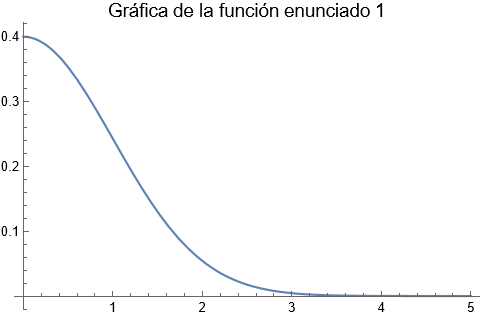
\includegraphics[scale=0.7]{plot_P1_Inciso_01.png}
    \caption{Gráfica para la función del inciso 1 del problema 1.}
\end{figure}

\begin{figure}[H]
    \centering
    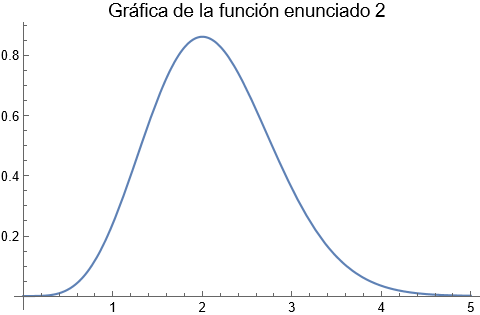
\includegraphics[scale=0.7]{plot_P1_Inciso_02.png}
    \caption{Gráfica para la función del inciso 2 del problema 1.}
\end{figure}
\item Tienes un valor exacto de la integral, el valor que te devuelve la técnica de Monte Carlo es la \emph{aproximación} o valor estimado.
\item La parte en donde se obtiene el valor de la integral y su error asociado está bien, pero hay detalles en la parte de graficación del método del dardo, ya que en tu ciclo \texttt{for}, se enciman las gráficas y no se aprecia precisamente como se van acumulando puntos por debajo de la gráfica y por arriba de ella. 
\item La rutina de graficación no queda claro el por qué haces algo distinto, si la función que utilizaste para calcular la integral te generaba el conjunto de datos aleatorios, básicamente lo que había que hacer es ocupar ese conjunto y graficarlo. Tu archivo experimental.py no ofrece propiamente una explicación y justificación de tu procedimiento, y como tal, no muestras las gráficas de puntos por debajo y por arriba de la curva.
\item \textbf{Calificación: 0.6}
\end{enumerate}

\section{Problema 2.}

\begin{enumerate}
\item Tu solución presenta una función que a partir de lo que llamas integración por el método de discos, no se justifica, recuerda que el enunciado menciona que tienes un hemisferio, como tal tienes una superficie en $(x, y, z)$ y lo reduces a un problema en el plano.
\item No discutes el cómo llegas a la expresión, que si bien presenta una curva, \texttt{no} es la curva esperada, por que no corresponde a lo que sería una parte del hemisferio. Esta discusión es la que te llevaría a plantear entonces la solución más pertinente.
\item ¿Cómo llegas al valor exacto del volumen del hemisferio? Se esperaba un manejo correspondiente de una integral triple con sus correspondientes límites de integración, es decir, un ejercicio que se resuelve del curso de Cálculo IV, pero que no se incluye en tu solución.
\item En la gráfica que tienes en la celda \emph{graficación de muestreo uniforme} tienes un resultado que no concuerda con lo que se pide, ya que el hemisferio es de radio unitario, la altura de la curva tendría que ser $1$ y en tu gráfica la llevaste a $3$, ¿qué pasó?
\item Lo que recomiendo es que siempre plantees de manera organizada tu problema: ¿qué se te pide? ¿qué es lo que tienes? ¿qué desarrollo haces? para entonces proponer una solución con algoritmos y de esa manera te será más fácil el trabajo.
\item \textbf{Calificación: 0.7}
\end{enumerate}

\end{document}